{
    {
        \newcommand{\tempwidth}[0]{0.8\linewidth}
        \begin{figure}
             \centering
             \begin{subfigure}{\textwidth}
                 \centering
                 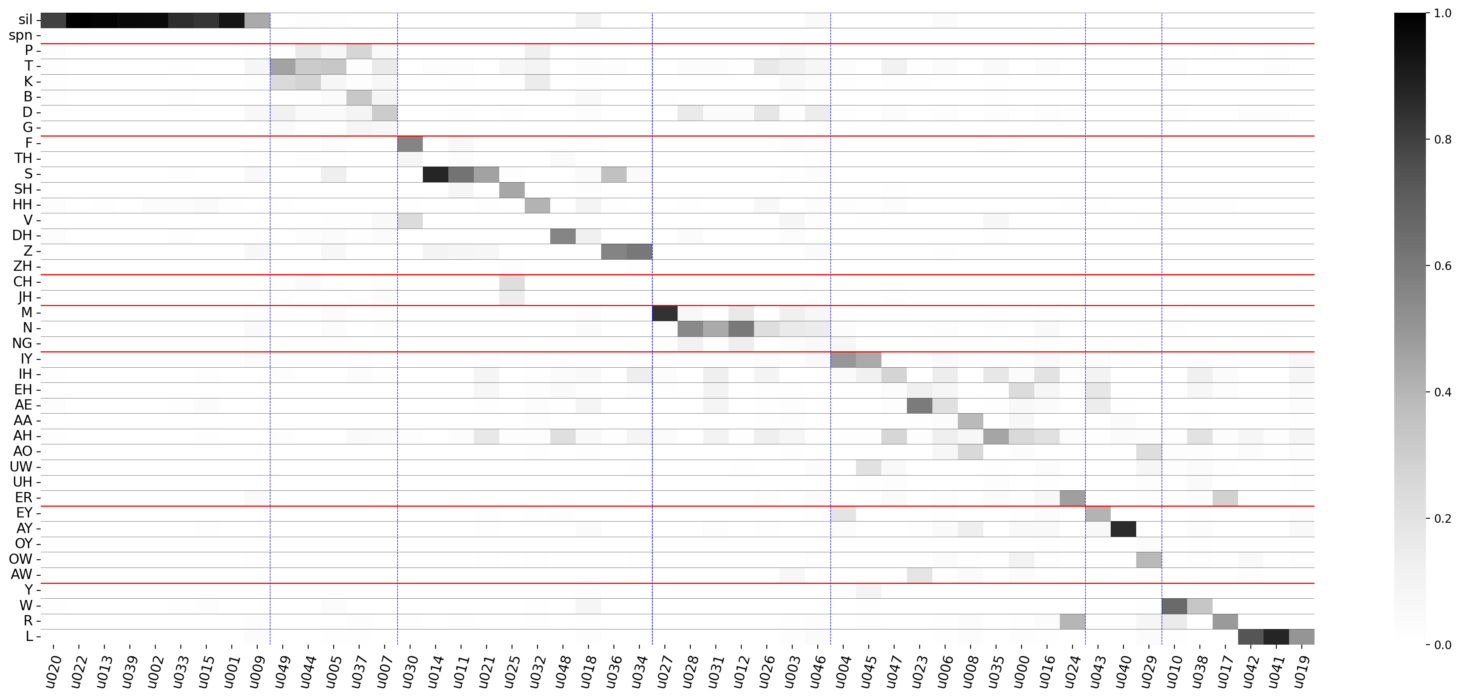
\includegraphics[width=\tempwidth]{figures/ch4figs/hub-u050-ap0000-givenunit-byphn.png}
                 \caption{離散單元}
                 \label{fig:hub-u050-ap0000-givenunit-byphn}
             \end{subfigure}
             \vfill
             \begin{subfigure}{\textwidth}
                 \centering
                 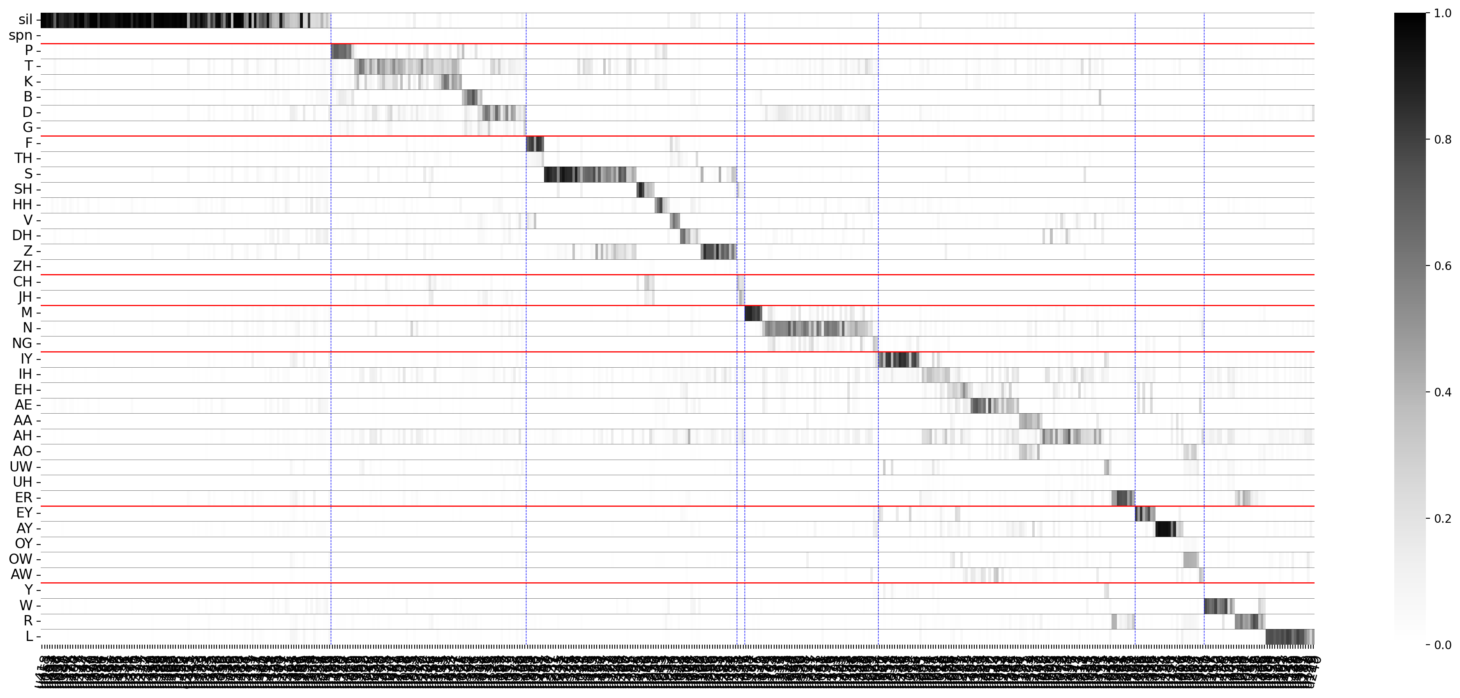
\includegraphics[width=\tempwidth]{figures/ch4figs/hub-u050-ap0500-givenunit-byphn.png}
                 \caption{500 種次詞單位}
                 \label{fig:hub-u050-ap0500-givenunit-byphn}
             \end{subfigure}
             \vfill
             \begin{subfigure}{\textwidth}
                 \centering
                 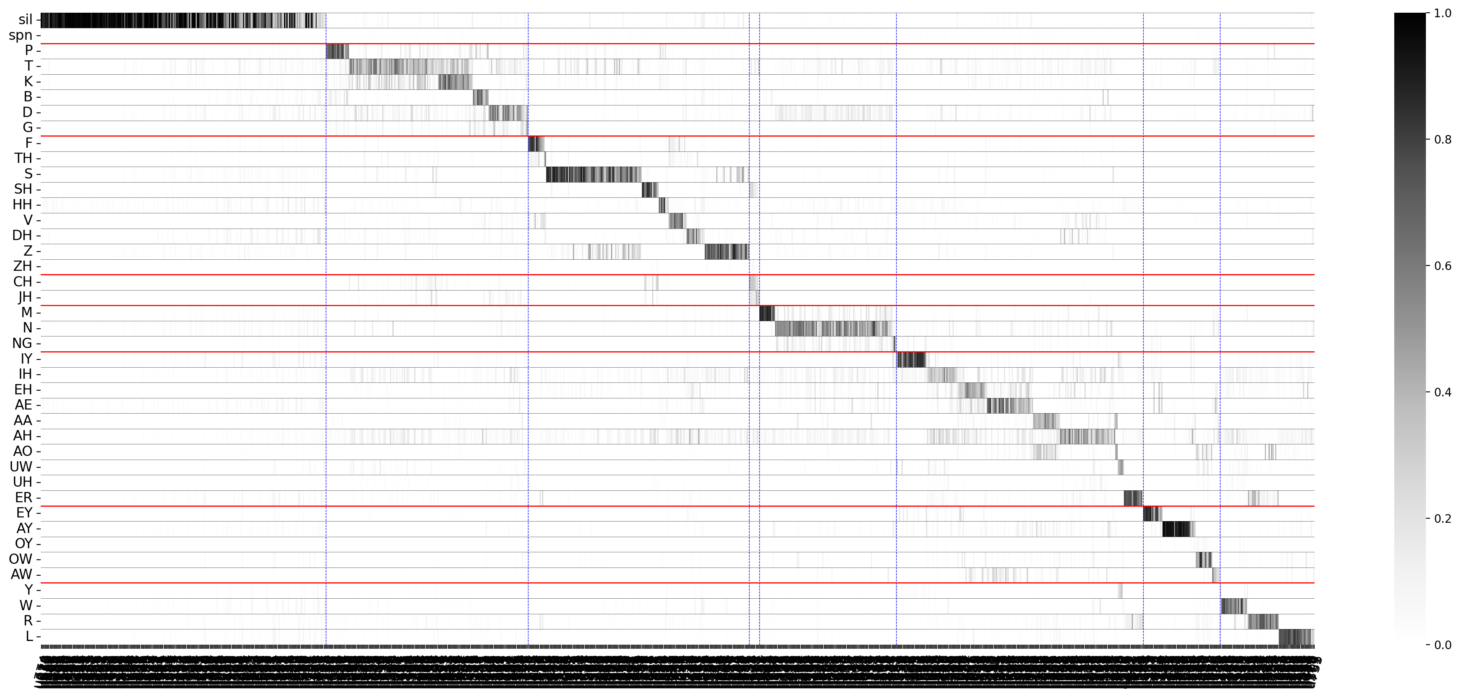
\includegraphics[width=\tempwidth]{figures/ch4figs/hub-u050-ap1000-givenunit-byphn.png}
                 \caption{1000 種次詞單位}
                 \label{fig:hub-u050-ap1000-givenunit-byphn}
             \end{subfigure}

             \caption{HuBERT 表徵在 K-平均演算法使用分群數 50 後,}
             比較不同次詞單位數量的條件機率分佈 $p_{y|z}(i | j)$ 熱圖
             \label{fig:hub-u050-comparisons}
        \end{figure}
    }
    {
        \newcommand{\tempwidth}[0]{0.8\linewidth}
        \begin{figure}
             \centering
             \begin{subfigure}{\textwidth}
                 \centering
                 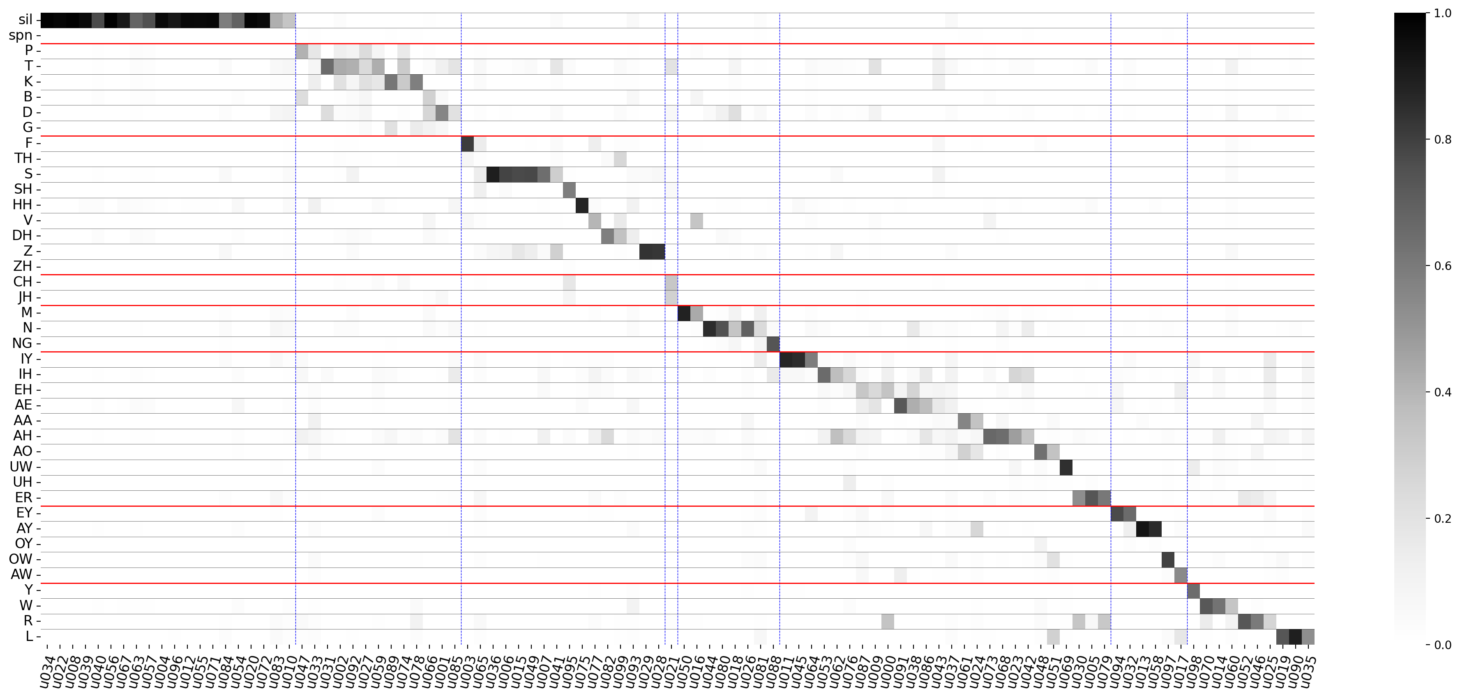
\includegraphics[width=\tempwidth]{figures/ch4figs/hub-u100-ap0000-givenunit-byphn.png}
                 \caption{離散單元}
                 \label{fig:hub-u100-ap0000-givenunit-byphn}
             \end{subfigure}
             \vfill
             \begin{subfigure}{\textwidth}
                 \centering
                 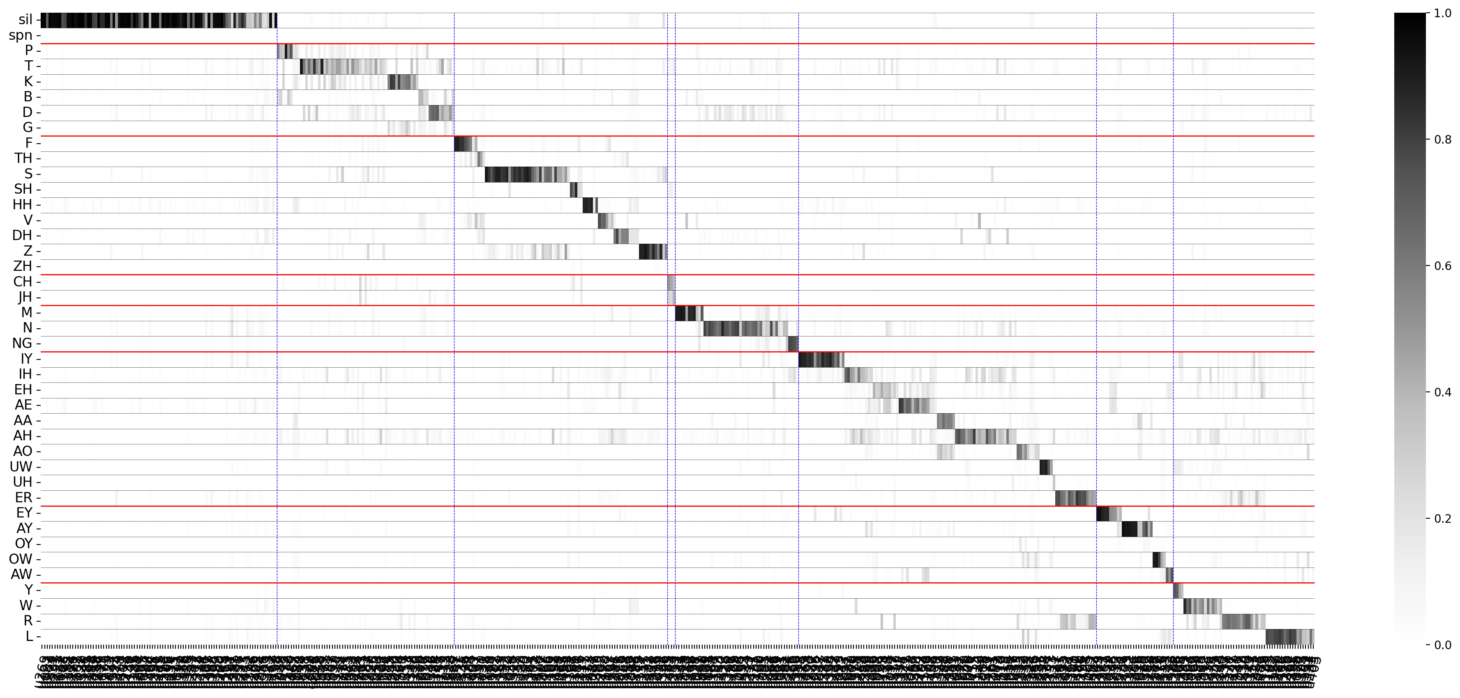
\includegraphics[width=\tempwidth]{figures/ch4figs/hub-u100-ap0500-givenunit-byphn.png}
                 \caption{500 種次詞單位}
                 \label{fig:hub-u100-ap0500-givenunit-byphn}
             \end{subfigure}
             \vfill
             \begin{subfigure}{\textwidth}
                 \centering
                 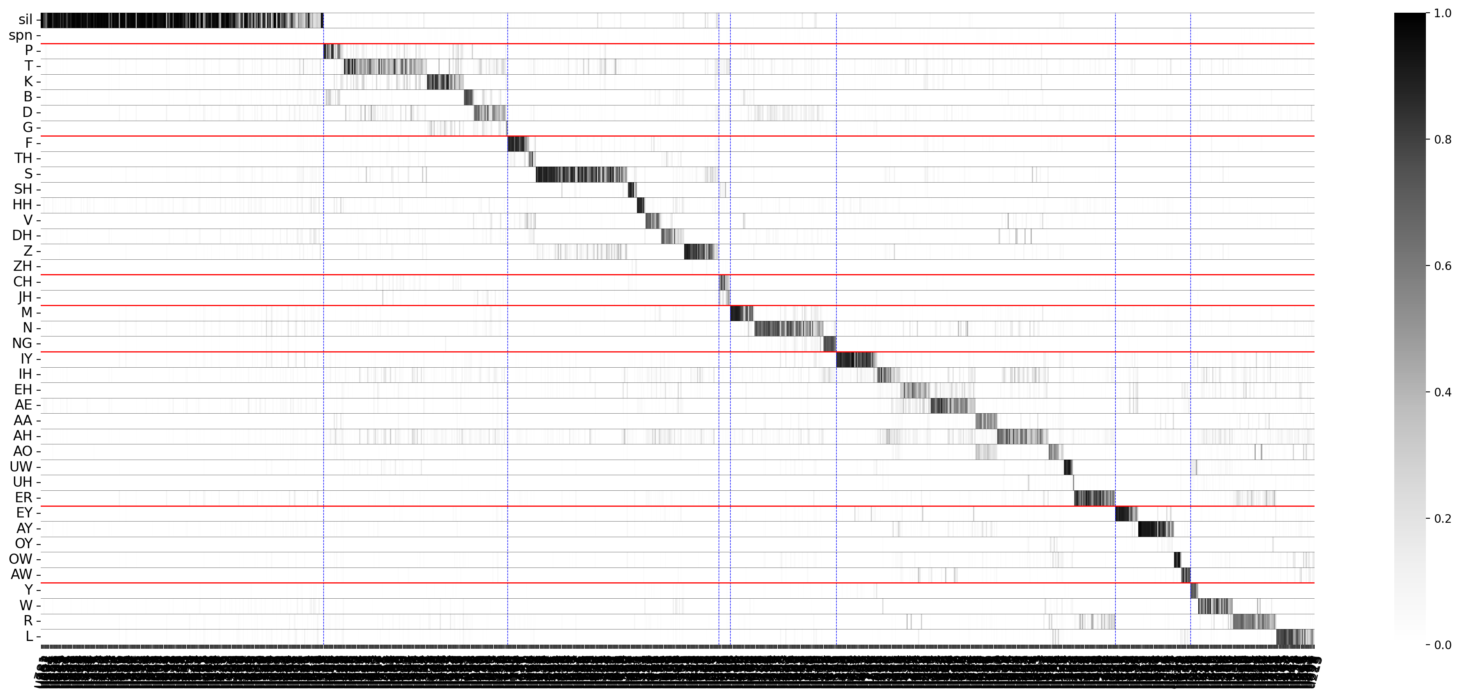
\includegraphics[width=\tempwidth]{figures/ch4figs/hub-u100-ap1000-givenunit-byphn.png}
                 \caption{1000 種次詞單位}
                 \label{fig:hub-u100-ap1000-givenunit-byphn}
             \end{subfigure}

             \caption{HuBERT 表徵在 K-平均演算法使用分群數 100 後,}
             比較不同次詞單位數量的條件機率分佈 $p_{y|z}(i | j)$ 熱圖
             \label{fig:hub-u100-comparisons}
        \end{figure}
    }
}
